\chapter{Resultados e Discussões}\label{chapter:resultados}

Nesta seção, apresento os resultados e discussões sobre a utilização do modelo proposto na classificação de imagens digitais de exames de Papanicolaou A base de dados consiste em imagens de 100 x 100 píxeis que foram redimensionadas para 50 x 50 píxels.O objetivo do modelo é distinguir entre células normais e anormais em imagens histopatológicas, explorando a eficácia da arquitetura desenvolvida, avaliando a precisão do modelo e discutir a aplicabilidade dos resultados para diagnósticos.

Após o treinamento, foi avaliado o desempenho do modelo nos conjuntos de treinamento e teste. Os resultados foram muito encorajadores: o modelo alcançou uma acurácia de aproximadamente 86.62\% nos dados de teste e 88.86\% nos dados de treinamento. A perda média foi de 31.04\% nos dados de teste e 26.85\% nos dados de treinamento, indicando uma boa capacidade de generalização.

\begin{figure}[H]
    \centering
    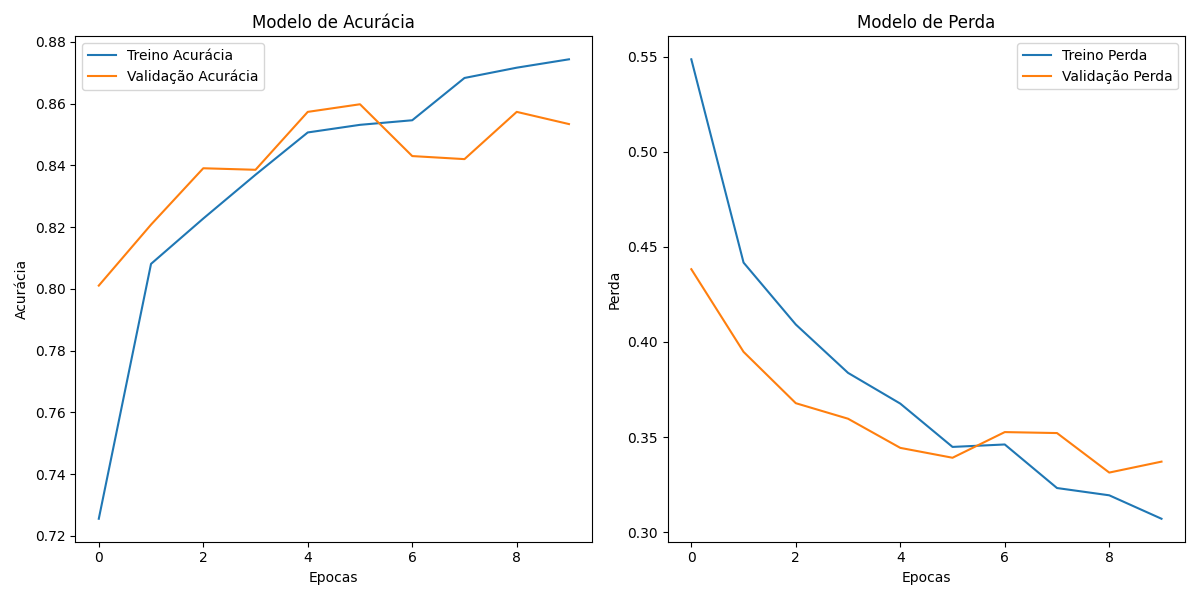
\includegraphics[width=1.0\textwidth]{figuras/modelos.png}
    \caption{Modelo de Acurácia e Perda.}
    \label{fig:nome_da_imagem}
\end{figure}

Além da acurácia e da perda, foi calculadas a precisão e a revocação do modelo. A precisão foi medida em 86.63\%, o que indica a proporção de instâncias positivas (células anormais) corretamente classificadas pelo modelo. A revocação também foi de 86.62\%, representando a capacidade do modelo de identificar todas as instâncias positivas.

\begin{figure}[H]
    \centering
    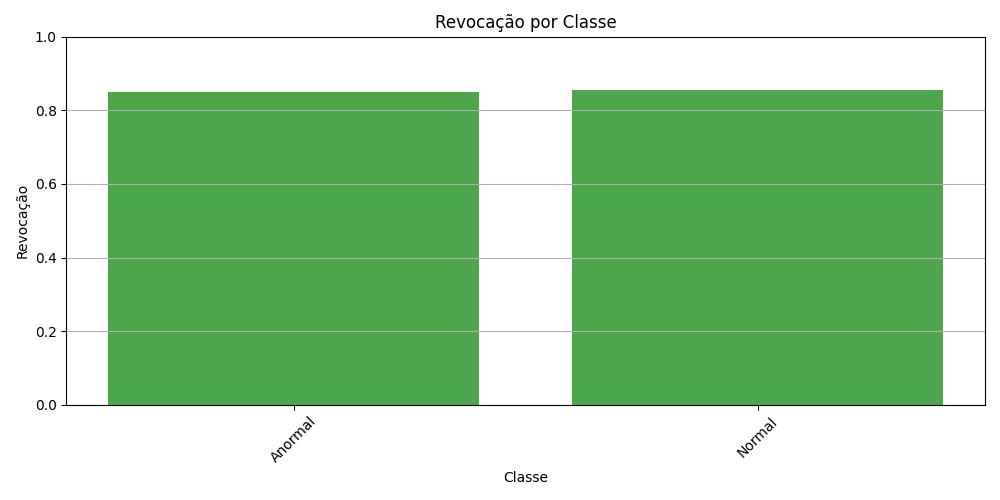
\includegraphics[width=1.0\textwidth]{figuras/revocacao.png}
    \caption{Revocação.}
    \label{fig:nome_da_imagem}
\end{figure}

\begin{figure}[H]
    \centering
    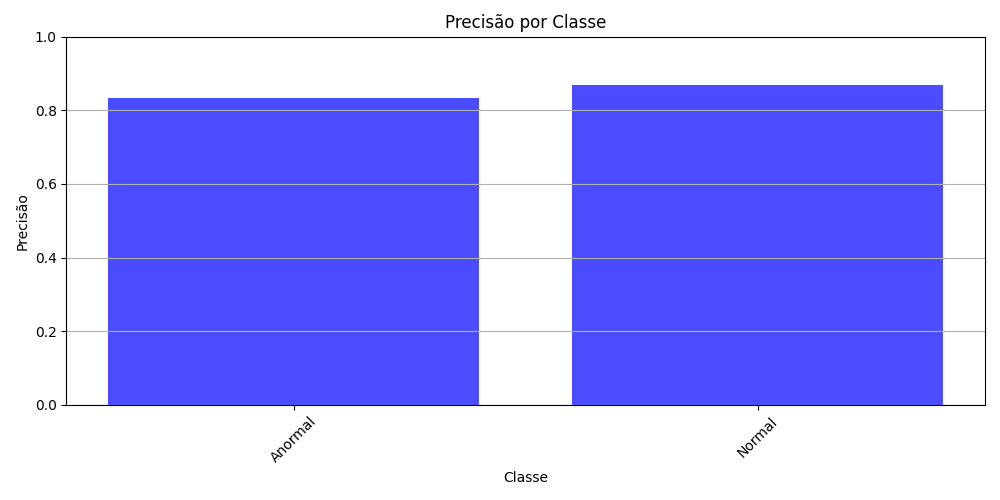
\includegraphics[width=1.0\textwidth]{figuras/precisao.png}
    \caption{Precisão.}
    \label{fig:nome_da_imagem}
\end{figure}

A matriz de confusão é uma ferramenta fundamental para a avaliação do desempenho de modelos de classificação, oferecendo uma visão detalhada sobre a eficácia do modelo em termos de suas previsões. No contexto deste estudo, onde foi desenvolvido um modelo de rede neural convolucional para classificar imagens de células cervicais como normais ou anormais, a matriz de confusão é apresentada da seguinte forma:

\begin{figure}[H]
    \centering
    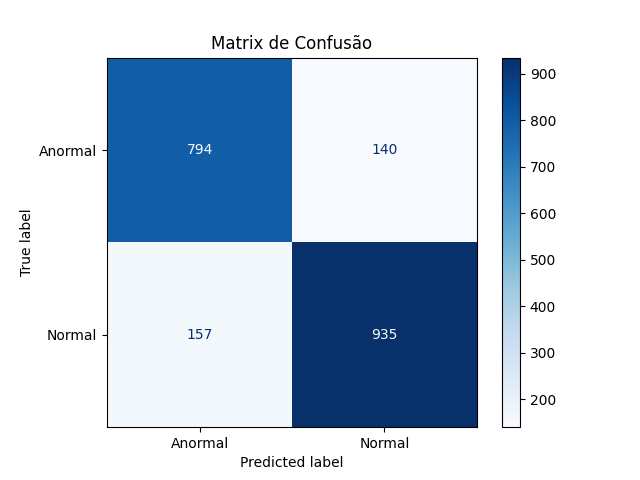
\includegraphics[width=1.0\textwidth]{figuras/matriz.png}
    \caption{Matriz de Confusão.}
    \label{fig:nome_da_imagem}
\end{figure}


Na matriz, podemos observar que o modelo obteve um bom desempenho geral, no entanto, o modelo teve algumas dificuldades em classificar corretamente as instâncias anormais. A matriz de confusão indica que o modelo é altamente eficaz na classificação das células cervicais, com alta precisão e revocação. As métricas calculadas sugerem que o modelo tem um bom equilíbrio entre a capacidade de identificar corretamente as amostras positivas e negativas.

A especificidade alta sugere uma forte habilidade do modelo em identificar corretamente as amostras negativas, crucial para minimizar falsos positivos em diagnósticos clínicos. O F1-Score consistente indica um equilíbrio robusto entre precisão e revocação, enquanto a variabilidade na especificidade pode sugerir áreas para otimização adicional do modelo.

\begin{figure}[H]
    \centering
    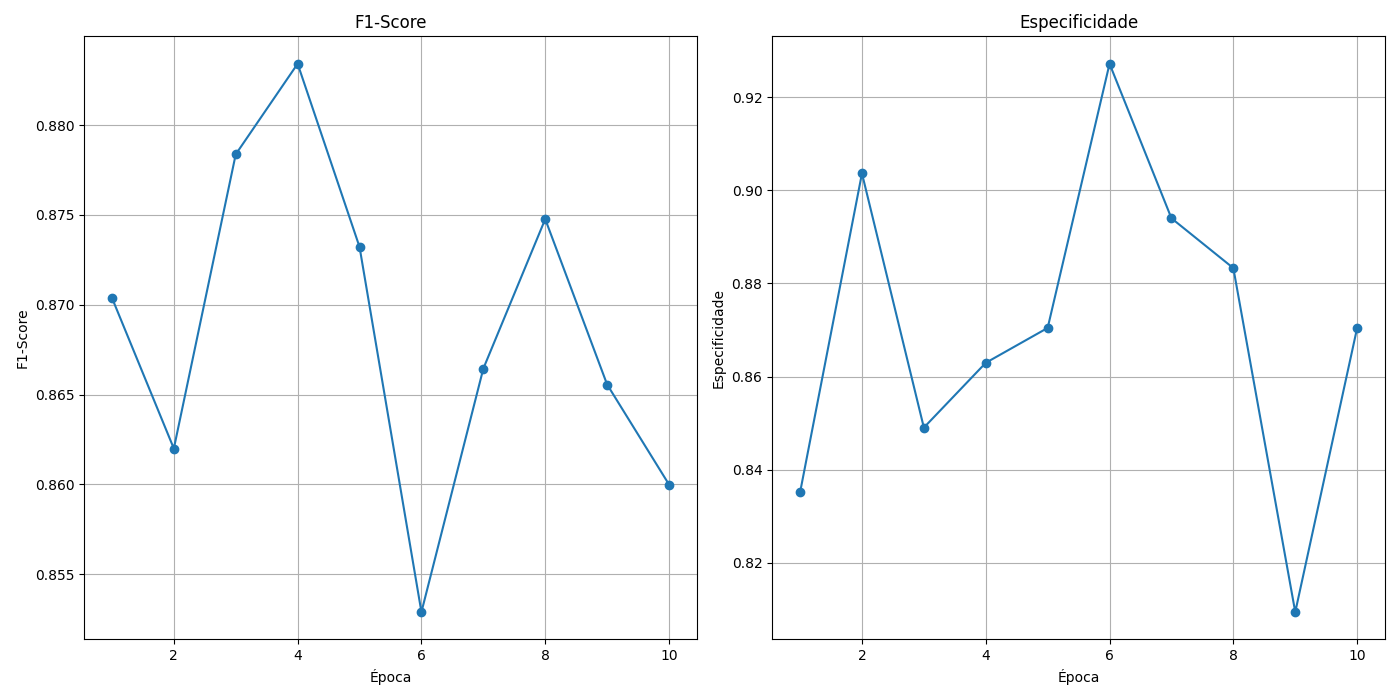
\includegraphics[width=1.0\textwidth]{figuras/F1_Esp.png}
    \caption{F1-SCORE e Especificidade.}
    \label{fig:nome_da_imagem}
\end{figure}
